\documentclass[english]{beamer}

% Packages
\usepackage[utf8]{inputenc}
\usepackage[margin=1in]{geometry}
\usepackage{amssymb}
% PDF metadata
\usepackage[pdftex]{hyperref}
% For figure alignment
\usepackage{float}
% For colored text
\usepackage{xcolor}
% For SI unit notation
\usepackage{siunitx}
% For diagrams
\usepackage{tikz}
\usetikzlibrary{arrows.meta}
\usetikzlibrary{patterns.meta}
\usetikzlibrary{positioning}
\tikzset{>={Stealth[length=2mm]}}
% For citations
\usepackage[backend=biber]{biblatex}
% Better quotations
\usepackage[style=english]{csquotes}
% Language and localization
\usepackage{babel}
% Fix special characters
\usepackage[T1]{fontenc}


% Misc settings
% Remove indentation
\setlength{\parindent}{0in}
% Set paragraph spacing
\setlength{\parskip}{12pt}


% Macros
% Mark placeholder fields
\newcommand{\todo}[1][TODO]{{\color{red}#1}}

\hypersetup{
	pdftitle = {%
		Efficient CNN Accelerators on FPGAs
	},
	pdfauthor = {Clarity Shimoniak},
	pdfsubject = {EE 243 Project Presentation},
	pdfkeywords = {%
		computer vision, convolutional neural network, CNN, FPGA, Xilinx,
		Lattice, MNIST
	},
}

\addbibresource{fpga.bib}
\addbibresource{models.bib}
\addbibresource{related.bib}


\begin{document}

\title{Efficient CNN Accelerators on FPGAs}
\subtitle{EE 243 Final Project}
\author{Clarity Shimoniak}
\date{Spring 2024}
\frame{\titlepage}


\begin{frame}
\frametitle{Problem Statement and Motivation}
\begin{itemize}
	\item FPGA accelerators are promising for embedded applications where GPUs
	are unavailable.
	\item Depthwise-separable convolutions are key to the efficiency of
	MobileNet\supercites{mobilenetv1}{mobilenetv2} \&
	EfficientNet\supercite{efficientnet}.
	\item Existing FPGA accelerators do not implement them efficiently.
	\item Most FPGA accelerators do not publicly release code.
	\begin{itemize}
		\item All rely on expensive, proprietary Altera or Xilinx boards.
	\end{itemize}
\end{itemize}
\end{frame}


\begin{frame}
\frametitle{Framework Overview Figure}
	\begin{columns}
		\column{0.5\linewidth}
		\begin{figure}
			\centering
			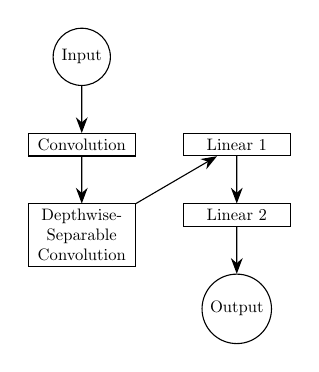
\begin{tikzpicture}[
				scale=0.6, transform shape,
				endpoint/.style = {
					circle, draw
				},
				layer/.style = {
					rectangle, draw,
					align=center,
					text width=0.8in
				}
			]
				\node[endpoint] (in) {Input};
				\node[layer, below=of in] (conv1) {Convolution};
				\node[layer, below=of conv1] (conv2)
					{Depthwise-Separable Convolution};
				\node[layer, right=of conv1] (fc1) {Linear 1};
				\node[layer, below=of fc1] (fc2) {Linear 2};
				\node[endpoint, below=of fc2] (out) {Output};
				\draw[->] (in) -- (conv1);
				\draw[->] (conv1) -- (conv2);
				\draw[->] (conv2) -- (fc1);
				\draw[->] (fc1) -- (fc2);
				\draw[->] (fc2) -- (out);
			\end{tikzpicture}
		\end{figure}
		\begin{itemize}
			\item Similar to early MobileNet stage.
			\item Trained with PyTorch on Colab.
			\begin{itemize}
				\item $\SI{90}{\percent}$ accuracy on MNIST.
			\end{itemize}
		\end{itemize}
	\end{columns}
\end{frame}


\begin{frame}
\frametitle{Methodology}
\begin{itemize}
	\item Create a small network with a similar architecture to MobileNet.
	\begin{itemize}
		\item Only open-source FPGA MobileNet
		accelerator\supercite{solovyev2019mobilenet} is dependent on
		proprietary \$700 board.
	\end{itemize}
	\item Use the DPU architecture proposed by
	\citeauthor{mobilenet2019fpga}\supercite{mobilenet2019fpga}
	to accelerate it.
	\begin{itemize}
		\item Compare against an un-optimized architecture for the same network.
	\end{itemize}
\end{itemize}
\end{frame}


\begin{frame}
\frametitle{Experiments \& Results}
\end{frame}


\begin{frame}[allowframebreaks]
\frametitle{References}
\tiny\printbibliography
\end{frame}


\end{document}
